\chapter{Множества, логика и доказательства}\label{chap:c16}\markright{Глава 9}
\begin{definition}\term{Множество} (\emph{set}) — совокупность элементов. Запись \(x \in  A\) означает, что \(x\) принадлежит множеству \(A\).\end{definition}
\begin{definition}\term{Пересечение} (\emph{intersection}) \(A\cap B\) — множество элементов, принадлежащих одновременно \(A\) и \(B\).\end{definition}
\begin{definition}\term{Объединение} (\emph{union}) \(A\cup B\) — множество элементов, принадлежащих хотя бы одному из множеств \(A\) и \(B\).\end{definition}
\begin{definition}\term{Утверждение} (\emph{statement; proposition}) — высказывание, для которого можно определить истинность или ложность в заданных условиях.\end{definition}
\begin{definition}\term{Импликация} (\emph{implication}) \(P\Rightarrow Q\) — высказывание «если \(P\), то \(Q\)».\end{definition}
\begin{definition}\term{Достаточное условие} (\emph{sufficient condition}) для \(Q\) — условие \(P\), из которого следует \(Q\), то есть импликация \(P\Rightarrow Q\) истинна.\end{definition}
\begin{definition}\term{Необходимое условие} (\emph{necessary condition}) для \(P\) — условие \(Q\), которое обязательно выполняется при выполнении \(P\), то есть импликация \(P\Rightarrow Q\) истинна.\end{definition}
\section{Кванторы и отрицание}
\par\addvspace{5pt}\begin{lrbox}{\CatFlowBox}\begin{minipage}[t]{\linewidth}
\setlength{\parskip}{5pt}\setlength{\columnsep}{4.5mm}\setlength{\intextsep}{0pt}
\begin{wrapfigure}[12]{r}{54mm}

\includegraphics[width=54mm,height=58mm,keepaspectratio]{images/unique/art-23.png}
\label{catflow:23}
\end{wrapfigure}
\(\forall \) означает «для любого», \(\exists \) — «существует». \(\mathbb{Z}\) обозначает целые числа, \(\mathbb{R}\) — действительные.\par
Отрицание «для всех \(x\) верно \(P (x)\)» — «существует \(x\), для которого \(P (x)\) неверно».\par
Чтобы опровергнуть всеобщее утверждение, достаточно одного контрпримера. Чтобы доказать его, проверки нескольких примеров недостаточно.\par
\par\WFclear\end{minipage}\end{lrbox}%
\ifdim\dimexpr\ht\CatFlowBox+\dp\CatFlowBox\relax<64mm\dp\CatFlowBox=\dimexpr64mm-\ht\CatFlowBox\relax\fi%
\noindent\usebox{\CatFlowBox}\par\addvspace{5pt}
\section{Свойства и способы доказательства}
Для конечных множеств: \(| A \cup  B | = | A | + | B | - | A \cap  B |\). Здесь \(| A |\) означает число элементов множества, а не модуль числа.\par
\begin{definition}\term{Контрапозиция} (\emph{contrapositive}) импликации \(P\Rightarrow Q\) — импликация \(\neg Q\Rightarrow\neg P\), равносильная исходной:\[ (P\Rightarrow Q)\Longleftrightarrow(\neg Q\Rightarrow\neg P). \] Здесь \(\neg\) означает отрицание.\end{definition}
Обратное утверждение \(Q\Rightarrow P\) в общем случае из \(P\Rightarrow Q\) не следует.\par
Принцип математической индукции: проверь утверждение для \(n = 1\); затем для любого \(k \ge  1\) докажи переход от его истинности при \(n = k\) к истинности при \(n = k + 1\). Тогда оно верно для всех натуральных \(n \ge  1\).\par
{\small\textit{Пример прямого доказательства: сумма чётных чисел \(2 m\) и \(2 n\) равна \(2 (m + n)\), поэтому она чётна.}}\par

\section{Подмножества и операции над множествами}
\begin{definition}\term{Подмножество} (subset) \(A\) множества \(B\) — множество, каждый элемент которого принадлежит \(B\). Обозначение \(A\subseteq B\) допускает равенство \(A=B\).\end{definition}
\begin{definition}\term{Собственное подмножество} (proper subset) — подмножество \(A\subseteq B\), не равное \(B\). Обозначение: \(A\subset B\). Здесь знак \(\subset\) всегда означает строгое включение; в литературе соглашения об этом знаке различаются.\end{definition}
\begin{definition}\term{Пустое множество} (empty set) \(\varnothing\) — множество, не содержащее ни одного элемента. Оно является подмножеством любого множества; \(\{\varnothing\}\) содержит один элемент и не равно \(\varnothing\).\end{definition}
\begin{definition}\term{Универсальное множество} (universal set) \(U\) — заранее выбранное множество всех объектов, рассматриваемых в данной задаче. Если говорится о дополнениях, все обсуждаемые множества считаются подмножествами \(U\).\end{definition}
\begin{definition}\term{Разность множеств} (set difference) \(A\setminus B\) — множество элементов, которые принадлежат \(A\), но не принадлежат \(B\).\end{definition}
\begin{definition}\term{Дополнение множества} (complement) \(A\subseteq U\) относительно \(U\) — множество \(U\setminus A\). Без указания \(U\) дополнение может быть неоднозначным.\end{definition}
\begin{definition}\term{Симметрическая разность} (symmetric difference) \(A\triangle B\) — множество элементов, принадлежащих ровно одному из множеств \(A,B\): \(A\triangle B=(A\setminus B)\cup(B\setminus A)\).\end{definition}
\begin{definition}\term{Множество всех подмножеств} (power set) множества \(A\) — множество \(\mathcal P(A)=\{B:B\subseteq A\}\). Например, \(\mathcal P(\{a\})=\{\varnothing,\{a\}\}\).\end{definition}
\begin{definition}\term{Упорядоченная пара} (ordered pair) \((a,b)\) — пара с выделенными первой и второй координатами: \((a,b)=(c,d)\) тогда и только тогда, когда \(a=c\) и \(b=d\).\end{definition}
\begin{definition}\term{Декартово произведение} (Cartesian product) \(A\times B\) — множество всех упорядоченных пар \((a,b)\), где \(a\in A\), \(b\in B\). Например, \(\{1,2\}\times\{3\}=\{(1,3),(2,3)\}\).\end{definition}
\begin{definition}\term{Диаграмма Венна} (Venn diagram) — рисунок, на котором универсальное множество изображают областью, обычно прямоугольником, а его подмножества — областями внутри неё. Закрашивание выделяет элементы, удовлетворяющие нужному условию. Диаграмма помогает понять равенство множеств, но общее доказательство удобно проводить через принадлежность произвольного элемента.\end{definition}
\begin{theorem}[Законы де Моргана]\label{thm:legacy-c16-1}
Если \(A,B\subseteq U\), то \(U\setminus(A\cup B)=(U\setminus A)\cap(U\setminus B)\) и \(U\setminus(A\cap B)=(U\setminus A)\cup(U\setminus B)\).
\end{theorem}
\begin{proof}
Возьмём произвольный \(x\in U\). Условие \(x\notin A\cup B\) означает, что \(x\notin A\) и \(x\notin B\), то есть \(x\in(U\setminus A)\cap(U\setminus B)\). Все переходы обратимы, поэтому доказано первое равенство. Условие \(x\notin A\cap B\) означает, что хотя бы одно из условий \(x\in A\), \(x\in B\) не выполнено. Это равносильно \(x\notin A\) или \(x\notin B\), то есть \(x\in(U\setminus A)\cup(U\setminus B)\). Обратимость переходов даёт второе равенство.
\end{proof}
\begin{theorem}[Число подмножеств]\label{thm:legacy-c16-2}
Если конечное множество \(A\) содержит \(n\) элементов, где \(n\ge0\) — целое число, то \(|\mathcal P(A)|=2^n\).
\end{theorem}
\par\addvspace{5pt}\begin{lrbox}{\CatFlowBox}\begin{minipage}[t]{\linewidth}
\setlength{\parskip}{5pt}\setlength{\columnsep}{4.5mm}\setlength{\intextsep}{0pt}
\begin{wrapfigure}[10]{l}{54mm}

\includegraphics[width=54mm,height=58mm,keepaspectratio]{images/unique/art-95.png}
\label{catflow:95}
\end{wrapfigure}
\textit{Доказательство.} Проведём индукцию по \(n\). При \(n=0\) множество \(A\) пусто и имеет ровно одно подмножество — \(\varnothing\); это \(1=2^0\). Пусть у множества из \(k\) элементов \(2^k\) подмножеств. При добавлении нового элемента каждое старое подмножество даёт два различных варианта: без нового элемента и с ним. Эти варианты исчерпывают все подмножества нового множества, поэтому их число равно \(2\cdot2^k=2^{k+1}\).\hfill\(\blacksquare\)
\par\WFclear\end{minipage}\end{lrbox}%
\ifdim\dimexpr\ht\CatFlowBox+\dp\CatFlowBox\relax<64mm\dp\CatFlowBox=\dimexpr64mm-\ht\CatFlowBox\relax\fi%
\noindent\usebox{\CatFlowBox}\par\addvspace{5pt}


\section{Логические связки и формулы}
Дальше изучаем двухзначную логику высказываний: каждое высказывание при заданных условиях имеет одно из двух истинностных значений. Обозначим истину числом \(1\), ложь числом \(0\). Это логические значения; арифметические действия с ними здесь не подразумеваются.

\begin{definition}\term{Пропозициональная переменная} (\emph{propositional variable}) — буква, обозначающая высказывание. Для переменных используем \(p,q,r,\ldots\), а для произвольных формул — \(A,B,C,\ldots\).\end{definition}
\begin{definition}\term{Логическая связка} (\emph{logical connective}) — операция, которая определяет истинностное значение составного высказывания по истинностным значениям его частей.\end{definition}
\begin{definition}\term{Константа истины} (\emph{truth constant}) \(\top\) имеет значение \(1\) при любых значениях переменных.\end{definition}
\begin{definition}\term{Константа лжи} (\emph{falsity constant}) \(\bot\) имеет значение \(0\) при любых значениях переменных.\end{definition}
\begin{definition}\term{Отрицание} (\emph{negation; NOT}) \(\neg A\) истинно ровно тогда, когда \(A\) ложно.\end{definition}
\begin{definition}\term{Конъюнкция} (\emph{conjunction; AND}) \(A\land B\) истинна ровно тогда, когда истинны обе части: и \(A\), и \(B\).\end{definition}
\begin{definition}\term{Дизъюнкция} (\emph{disjunction; OR}) \(A\lor B\) истинна, когда истинна хотя бы одна из частей, в том числе когда истинны обе.\end{definition}
\begin{definition}\term{Исключающее или} (\emph{exclusive OR; XOR}) \(A\oplus B\) истинно, когда истинна ровно одна из частей.\end{definition}
\begin{definition}\term{Материальная импликация} (\emph{material implication}) \(A\to B\) ложна только в случае, когда \(A\) истинно, а \(B\) ложно. Во всех остальных случаях она истинна.\end{definition}
Для импликации внутри формул этого раздела используем \(\to\); ранее в записях «если \(P\), то \(Q\)» использовалось обозначение \(\Rightarrow\). Истинность импликации сама по себе не утверждает причинной связи. Если условие \(A\) ложно, импликация \(A\to B\) истинна при любом значении \(B\); это не означает, что \(B\) истинно.
\begin{definition}\term{Бикондиционал} (\emph{biconditional; if and only if, iff}) \(A\leftrightarrow B\) истинен ровно тогда, когда \(A\) и \(B\) имеют одинаковые истинностные значения. Его читают «\(A\) тогда и только тогда, когда \(B\)».\end{definition}
\begin{definition}\term{Штрих Шеффера} (\emph{Sheffer stroke; NAND}) \(A\uparrow B\) — отрицание конъюнкции: \(\neg(A\land B)\).\end{definition}
\begin{definition}\term{Стрелка Пирса} (\emph{Peirce arrow; NOR}) \(A\downarrow B\) — отрицание дизъюнкции: \(\neg(A\lor B)\).\end{definition}

\begin{definition}\term{Пропозициональная формула} (\emph{propositional formula}) — конечная запись, построенная по следующим правилам. Каждая переменная, а также \(\top,\bot\) — формулы. Если \(A,B\) — формулы, то \(\neg A\) и \((A\circ B)\) — формулы для любой из связок \(\circ\in\{\land,\lor,\oplus,\to,\leftrightarrow,\uparrow,\downarrow\}\). Других способов построения формул нет.\end{definition}
Скобки указывают порядок применения связок. Внешние скобки можно опускать; \(\neg\) относится к ближайшей следующей формуле. При возможной неоднозначности скобки сохраняем: \(\neg(p\lor q)\) и \((\neg p)\lor q\) — разные формулы.
\begin{definition}\term{Оценка истинности} (\emph{truth assignment; valuation}) \(v\) приписывает каждой переменной значение \(0\) или \(1\). Значение \(v(A)\) составной формулы получают из значений её частей по определениям связок. Запись \(v\models A\) означает \(v(A)=1\).\end{definition}
\begin{definition}\term{Таблица истинности} (\emph{truth table}) — таблица, которая перечисляет все наборы значений входных переменных и соответствующие значения формул. Для \(n\) различных переменных существует \(2^n\) строк с входными наборами.\end{definition}

\begin{center}
\begin{tabular}{|c|c|}
\hline
\(A\)&\(\neg A\)\\ \hline
\(0\)&\(1\)\\ \hline
\(1\)&\(0\)\\ \hline
\end{tabular}
\end{center}
Следующая таблица задаёт все семь бинарных связок. В первых двух колонках находятся входные значения, в остальных — результаты операций.
\begin{center}
\begingroup\small\setlength{\tabcolsep}{5pt}
\begin{tabular}{|c|c|c|c|c|c|c|c|c|}
\hline
\(A\)&\(B\)&\(A\land B\)&\(A\lor B\)&\(A\oplus B\)&\(A\to B\)&\(A\leftrightarrow B\)&\(A\uparrow B\)&\(A\downarrow B\)\\ \hline
\(0\)&\(0\)&\(0\)&\(0\)&\(0\)&\(1\)&\(1\)&\(1\)&\(1\)\\ \hline
\(0\)&\(1\)&\(0\)&\(1\)&\(1\)&\(1\)&\(0\)&\(1\)&\(0\)\\ \hline
\(1\)&\(0\)&\(0\)&\(1\)&\(1\)&\(0\)&\(0\)&\(1\)&\(0\)\\ \hline
\(1\)&\(1\)&\(1\)&\(1\)&\(0\)&\(1\)&\(1\)&\(0\)&\(0\)\\ \hline
\end{tabular}
\endgroup
\end{center}

\par\addvspace{5pt}\begin{lrbox}{\CatFlowBox}\begin{minipage}[t]{\linewidth}
\setlength{\parskip}{5pt}\setlength{\columnsep}{4.5mm}\setlength{\intextsep}{0pt}
\begin{wrapfigure}[11]{l}{54mm}
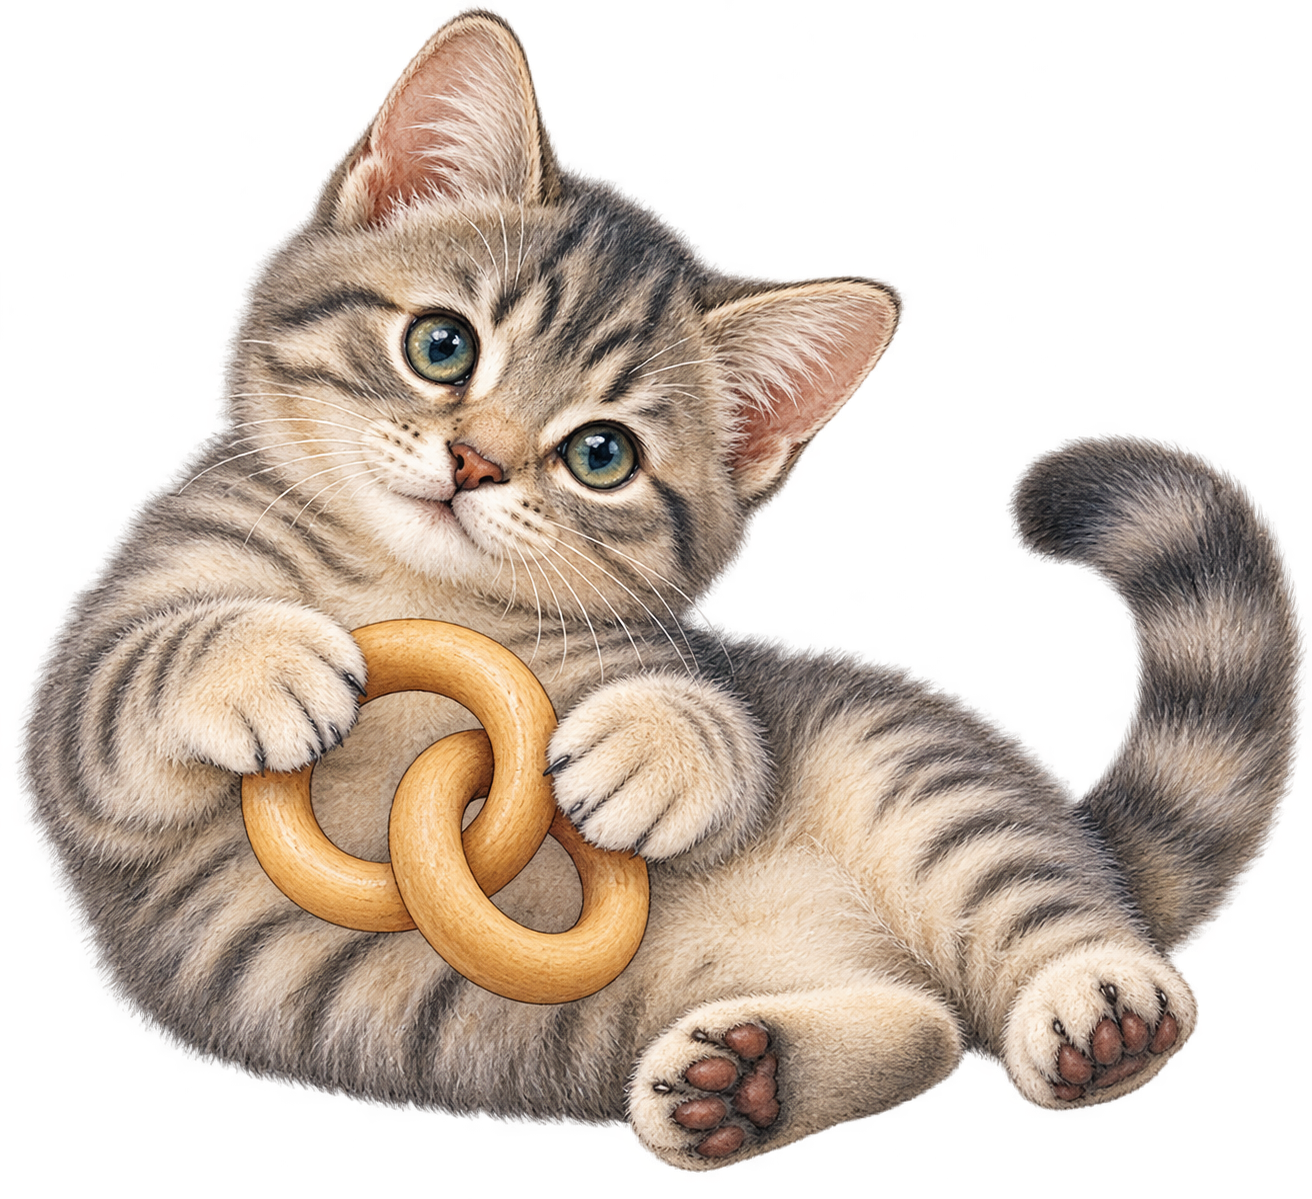
\includegraphics[width=54mm,height=58mm,keepaspectratio]{images/unique/art-81.png}
\label{catflow:81}
\end{wrapfigure}
Логический переключатель хранит только одно из двух состояний. Даже когда буквы обозначают сложные события, связка видит лишь их истинностные значения. Поэтому одна таблица подходит и для математических утверждений, и для условий доступа, и для модели электрической схемы. При переводе обычной фразы сначала выясни смысл слова «или»: допускаются оба события или требуется ровно одно. Затем назначь буквы простым утверждениям и расставь скобки. Полученная формула позволяет проверять конкретные ситуации, но её соответствие исходной фразе всё равно нужно обосновать словами.
\par\WFclear\end{minipage}\end{lrbox}%
\ifdim\dimexpr\ht\CatFlowBox+\dp\CatFlowBox\relax<64mm\dp\CatFlowBox=\dimexpr64mm-\ht\CatFlowBox\relax\fi%
\noindent\usebox{\CatFlowBox}\par\addvspace{5pt}
\section{Равносильность и семантическое следование}
\begin{definition}\term{Тавтология} (\emph{tautology}) — формула, истинная при каждой оценке её переменных. Например, \(p\lor\neg p\).\end{definition}
\begin{definition}\term{Противоречие} (\emph{contradiction}) — формула, ложная при каждой оценке её переменных. Например, \(p\land\neg p\).\end{definition}
Формула может не быть ни тавтологией, ни противоречием: \(p\land q\) принимает оба истинностных значения при разных оценках.
\begin{definition}\term{Логическая равносильность} (\emph{logical equivalence}) формул \(A,B\) означает, что \(v(A)=v(B)\) при каждой оценке \(v\). В этом разделе обозначаем её \(A\equiv B\).\end{definition}
Запись \(A\leftrightarrow B\) является формулой, которой можно приписать значение при одной оценке. Запись \(A\equiv B\) — утверждение о двух формулах и \emph{всех} оценках. Например, при \(v(p)=v(q)=1\) бикондиционал \(p\leftrightarrow q\) истинен, но \(p\not\equiv q\): оценка \(v(p)=1,v(q)=0\) различает их.

\begin{theorem}[Основные логические равносильности]\label{thm:legacy-c16-3}
Для любых формул \(A,B\) справедливы
\[
\begin{aligned}
\neg\neg A&\equiv A,\\
\neg(A\land B)&\equiv(\neg A)\lor(\neg B),\\
\neg(A\lor B)&\equiv(\neg A)\land(\neg B),\\
A\to B&\equiv(\neg A)\lor B,\\
A\leftrightarrow B&\equiv(A\to B)\land(B\to A).
\end{aligned}
\]
Вторую и третью равносильности называют законами де Моргана для высказываний.
\end{theorem}
\begin{proof}
Двойное отрицание дважды меняет значение и возвращает исходное. Отрицание конъюнкции истинно, когда хотя бы одна часть ложна; отрицание дизъюнкции — когда ложны обе. Формулы \(A\to B\) и \((\neg A)\lor B\) обе ложны только при значениях \(A=1,B=0\). Две встречные импликации одновременно истинны ровно при одинаковых значениях частей. Все рассуждения применимы к каждой оценке, что и доказывает равносильности.
\end{proof}

\begin{theorem}[Законы исключающего или]\label{thm:legacy-c16-4}
Для любых формул \(A,B,C\)
\[
\begin{aligned}
A\oplus B&\equiv(A\lor B)\land\neg(A\land B),\\
A\oplus B&\equiv B\oplus A,\\
(A\oplus B)\oplus C&\equiv A\oplus(B\oplus C),\\
A\oplus A&\equiv\bot,\qquad A\oplus\bot\equiv A,\\
A\oplus\top&\equiv\neg A.
\end{aligned}
\]
\end{theorem}
\begin{proof}
В первой строке требуется хотя бы одна истинная часть и запрещены две истинные части: остаётся ровно одна. Перестановка частей этого условия не меняет. Для трёх частей обе расстановки скобок дают \(1\), когда истинна ровно одна из трёх частей или все три, и дают \(0\) в остальных случаях. Наконец, две одинаковые части не могут иметь разные значения, сравнение с \(0\) сохраняет значение, а сравнение с \(1\) меняет его. Это доказывает все строки.
\end{proof}

\begin{definition}\term{Семантическое следование} (\emph{semantic entailment}) \(\Gamma\models A\), где \(\Gamma\) — конечное множество формул, означает: при каждой оценке, делающей истинными \emph{все} формулы из \(\Gamma\), формула \(A\) тоже истинна.\end{definition}
Формулы из \(\Gamma\) называют \term{посылками} (\emph{premises}), а \(A\) — \term{заключением} (\emph{conclusion}). Запись \(v\models\Gamma\) сокращает условие \(v(B)=1\) для всех \(B\in\Gamma\). Для пустого множества посылок пишут \(\models A\); это означает, что \(A\) — тавтология. По определению \(A\equiv B\) равносильно тому, что \(\models(A\leftrightarrow B)\).

Чтобы опровергнуть следование, достаточно \term{контроценки} (\emph{countervaluation; countermodel}) — оценки, при которой все посылки истинны, а заключение ложно. Например, \(\{p\lor q\}\not\models p\): подойдут \(v(p)=0,v(q)=1\). Если ни одна оценка не делает все посылки истинными, условие \(\Gamma\models A\) выполнено для любой формулы \(A\): оценки с истинными посылками и ложным заключением нет.

\section{Секвенции и конечные деревья вывода}
\begin{definition}\term{Секвенция} (\emph{sequent}) — запись вида \(\Gamma\vdash A\), где слева находится конечное множество формул-посылок, а справа одна формула-заключение. Такая запись задаёт цель: получить \(A\) из посылок \(\Gamma\) по выбранным правилам вывода.\end{definition}
Пишем \(\Gamma,A\) вместо \(\Gamma\cup\{A\}\); порядок посылок и их повторения здесь не имеют значения. Если посылок нет, \(\varnothing\vdash A\) сокращаем до \(\vdash A\). Секвенцию можно предложить как цель; доказанной она становится после построения допустимого вывода.

\begin{definition}\term{Конечное дерево доказательства} (\emph{finite proof tree; derivation tree}) — конечное дерево с секвенциями в вершинах. В листьях стоят разрешённые начальные секвенции, а каждый переход от верхних вершин к нижней является применением одного из объявленных правил. Нижняя вершина, или корень, содержит доказываемую секвенцию.\end{definition}
\begin{definition}\term{Выводимость} (\emph{derivability}) \(A\) из \(\Gamma\) означает существование такого конечного дерева с корнем \(\Gamma\vdash A\). Когда утверждаем выводимость, запись \(\Gamma\vdash A\) означает именно существование дерева, а не результат проверки таблицы истинности.\end{definition}

\par\addvspace{5pt}\begin{lrbox}{\CatFlowBox}\begin{minipage}[t]{\linewidth}
\setlength{\parskip}{5pt}\setlength{\columnsep}{4.5mm}\setlength{\intextsep}{0pt}
\begin{wrapfigure}[11]{r}{54mm}
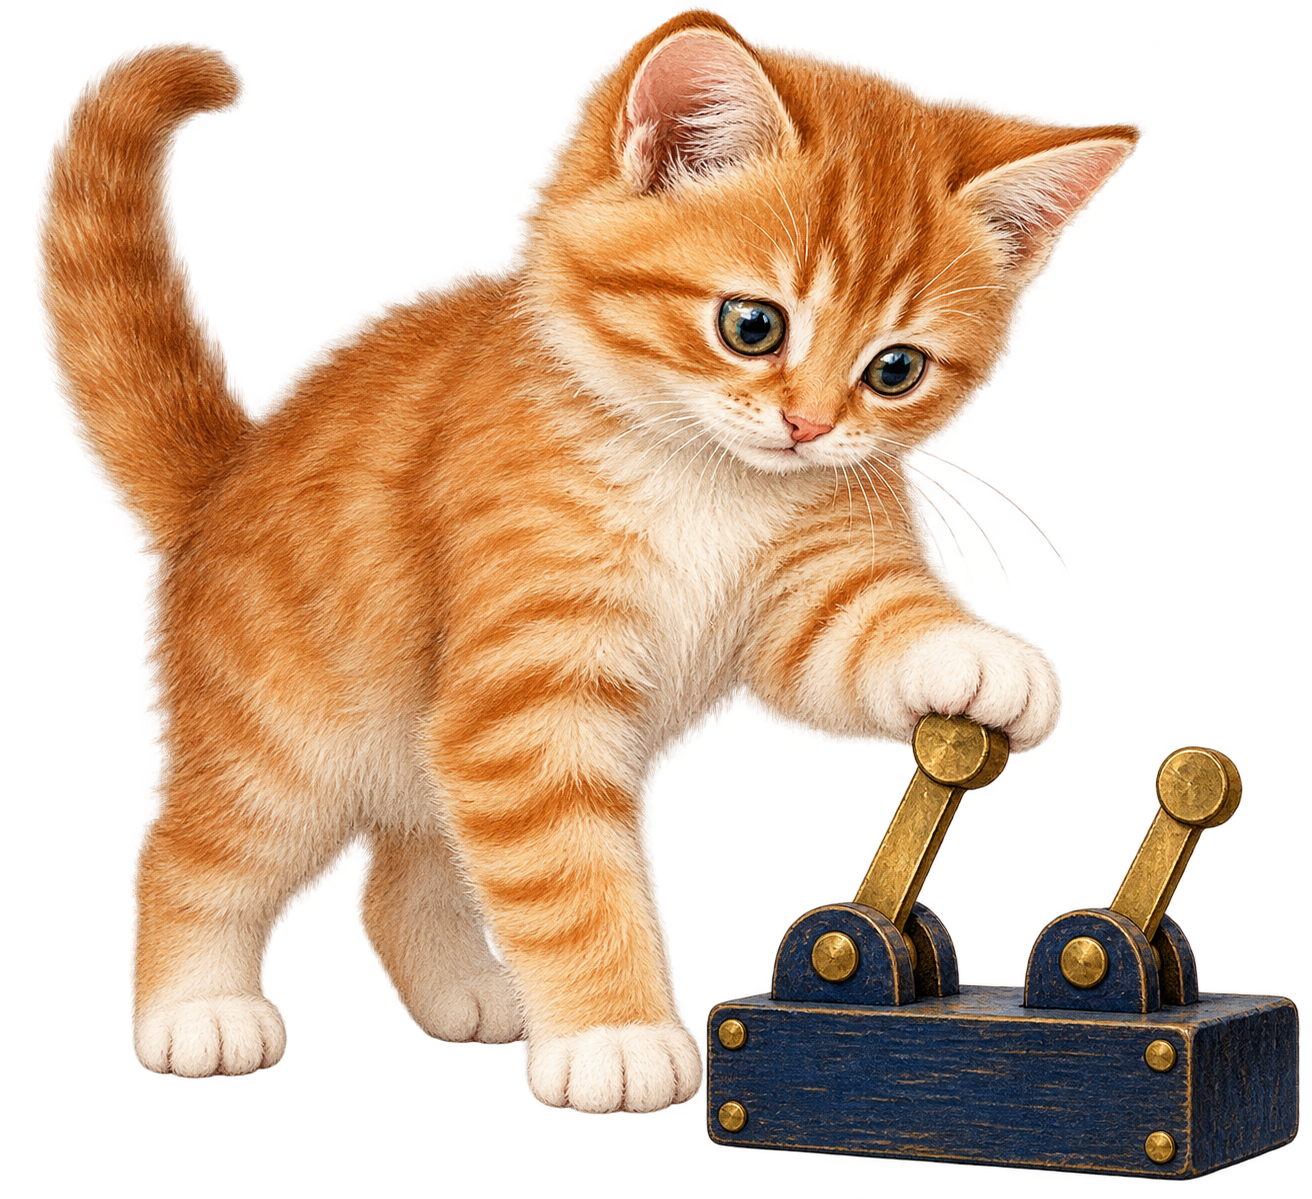
\includegraphics[width=54mm,height=58mm,keepaspectratio]{images/unique/art-82.png}
\label{catflow:82}
\end{wrapfigure}
Дерево вывода удобно читать от цели к основаниям. Нижняя строка показывает, что требуется получить, а правило подсказывает, какие более простые выводы нужно построить выше. При проверке движутся в обратную сторону: начинают с разрешённых предположений и проверяют каждый переход вниз. Временные предположения требуют отдельного внимания. Они помогают построить ветвь рассуждения, но их нельзя незаметно оставить среди безусловных фактов. Снятие предположения видно в изменении левой части секвенции; после этого заключение выражает, что удалось установить при данном условии.
\par\WFclear\end{minipage}\end{lrbox}%
\ifdim\dimexpr\ht\CatFlowBox+\dp\CatFlowBox\relax<64mm\dp\CatFlowBox=\dimexpr64mm-\ht\CatFlowBox\relax\fi%
\noindent\usebox{\CatFlowBox}\par\addvspace{5pt}
\subsection{Выбранные правила натурального вывода}
\term{Натуральный вывод} (\emph{natural deduction}) — способ строить доказательства введением и устранением логических связок. Здесь \(\vdash\) относится к следующему явно выбранному учебному набору правил для \(\land,\lor,\to\). В схемах \(A,B,C\) могут быть любыми формулами, а \(\Gamma\) — любым конечным множеством посылок. Доказательства табличных равносильностей выше являются семантическими.

\term{Правило предположения} (\emph{assumption rule}, \(\mathrm{Ax}\)):
\[
\frac{}{\Gamma\vdash A}\;(\mathrm{Ax}),\qquad A\in\Gamma.
\]
Любая объявленная посылка доступна без дополнительных шагов. Это начальная секвенция — лист дерева.

\term{Введение конъюнкции} (\emph{conjunction introduction}, \(\land I\)):
\[
\frac{\Gamma\vdash A\qquad\Gamma\vdash B}{\Gamma\vdash A\land B}\;(\land I).
\]
\term{Устранение конъюнкции} (\emph{conjunction elimination}):
\[
\frac{\Gamma\vdash A\land B}{\Gamma\vdash A}\;(\land E_1),
\qquad
\frac{\Gamma\vdash A\land B}{\Gamma\vdash B}\;(\land E_2).
\]

\term{Устранение импликации} (\emph{implication elimination; modus ponens}):
\[
\frac{\Gamma\vdash A\to B\qquad\Gamma\vdash A}{\Gamma\vdash B}\;(\to E).
\]
Для этого правила нужны и импликация, и её условие; одного заключения \(B\) недостаточно, чтобы восстановить \(A\).

\term{Введение импликации} (\emph{implication introduction}):
\[
\frac{\Gamma,A\vdash B}{\Gamma\vdash A\to B}\;(\to I).
\]
На верхнем этапе \(A\) добавлено как временное предположение. Внизу получена условная формула \(A\to B\), и добавленное предположение \term{снято} (\emph{discharged}). Исходные посылки из \(\Gamma\) сохраняются; если \(A\) уже входило в \(\Gamma\), оно остаётся исходной посылкой и после этого шага. Использовать временное предположение в верхней ветви необязательно.

\term{Введение дизъюнкции} (\emph{disjunction introduction}):
\[
\frac{\Gamma\vdash A}{\Gamma\vdash A\lor B}\;(\lor I_1),
\qquad
\frac{\Gamma\vdash B}{\Gamma\vdash A\lor B}\;(\lor I_2).
\]
\term{Устранение дизъюнкции} (\emph{disjunction elimination; proof by cases}):
\[
\frac{\Gamma\vdash A\lor B\qquad
      \Gamma,A\vdash C\qquad
      \Gamma,B\vdash C}
     {\Gamma\vdash C}\;(\lor E).
\]
Нужно получить одно и то же \(C\) в обоих случаях. Добавленное \(A\) снимают в первой ветви, добавленное \(B\) — во второй; исходные посылки \(\Gamma\) остаются.

\begin{theorem}[Выбранные правила сохраняют истину]\label{thm:legacy-c16-5}
Если \(\Gamma\vdash A\) имеет вывод по перечисленным правилам, то \(\Gamma\models A\).
\end{theorem}
\begin{proof}
Проведём индукцию по высоте конечного дерева. В листе правило \(\mathrm{Ax}\) выбирает одну из посылок, поэтому она истинна при каждой оценке, делающей истинным всё \(\Gamma\). Предположим, что утверждение уже верно для верхних поддеревьев.

Введение и устранение конъюнкции сохраняют истину по определению «и». Введение дизъюнкции сохраняет истину по определению «или». Для modus ponens истинность \(A\) и \(A\to B\) исключает единственный ложный случай импликации, поэтому \(B\) истинно.

При введении импликации возьмём оценку с истинными исходными посылками \(\Gamma\). Если \(A\) ложно, \(A\to B\) истинно. Если \(A\) истинно, верхнее поддерево с посылками \(\Gamma,A\) по индукционному предположению даёт истинность \(B\), и импликация снова истинна.

При разборе случаев истинная дизъюнкция делает истинной хотя бы одну из частей. Соответствующее верхнее поддерево с добавленным \(A\) или \(B\) даёт истинность \(C\). Таким образом, каждый допустимый последний шаг сохраняет истину, и индукция завершена.
\end{proof}
Следование \(\models\) говорит обо всех оценках, выводимость \(\vdash\) — о существовании конечного дерева в выбранной системе правил. Теорема устанавливает переход от построенного вывода к семантическому следованию. Таблица истинности подтверждает семантическое утверждение; чтобы предъявить формальный вывод, нужно указать дерево или последовательность шагов с их правилами.

\begin{theorem}[Перестановка двух условий]\label{thm:legacy-c16-6}
В выбранной системе выводима формула
\[
\vdash(p\land q)\to(q\land p).
\]
\end{theorem}
\begin{proof}
Временно предположим \(p\land q\) и обозначим \(\Delta=\{p\land q\}\). Правило предположения даёт \(\Delta\vdash p\land q\). Устранение конъюнкции даёт отдельно \(q\) и \(p\); введение конъюнкции соединяет их в обратном порядке:
\[
\frac{
 \displaystyle\frac{\Delta\vdash p\land q}{\Delta\vdash q}\;(\land E_2)
 \qquad
 \displaystyle\frac{\Delta\vdash p\land q}{\Delta\vdash p}\;(\land E_1)
}{
 \Delta\vdash q\land p
}\;(\land I).
\]
Две верхние секвенции — листья \(\mathrm{Ax}\) с одной и той же посылкой. Теперь снимаем временное предположение введением импликации:
\[
\frac{\{p\land q\}\vdash q\land p}
{\varnothing\vdash(p\land q)\to(q\land p)}\;(\to I).
\]
После этого открытых посылок не осталось. Каждый шаг указан явно; по предыдущей теореме полученная формула является также тавтологией.
\end{proof}

\section{Примеры: операции и отрицание}
\begin{example}Пусть \(A=\{1,2,3\}\), \(B=\{2,3,4\}\). Тогда \(A\cap B=\{2,3\}\), \(A\cup B=\{1,2,3,4\}\), \(A\setminus B=\{1\}\), \(A\mathbin{\triangle}B=\{1,4\}\). Принадлежность симметрической разности означает, что истинно ровно одно из условий \(x\in A\), \(x\in B\); это исключающее «или».\end{example}
\begin{example}Утверждение \(\forall x\in\mathbb R\quad x^2\ge x\) ложно: \(x=\frac12\) даёт \(\frac14<\frac12\). Его отрицание --- \(\exists x\in\mathbb R\quad x^2<x\). Для опровержения всеобщего утверждения достаточно одного свидетеля, но для его доказательства примера недостаточно.\end{example}
\Needspace{7\baselineskip}\section*{Задачи}
\begingroup\setlength{\parskip}{2pt}
\noindent\begin{minipage}[t]{\linewidth}\textbf{9.1.} При \(A = \{1,\allowbreak 2,\allowbreak 3\}\) и \(B = \{3,\allowbreak 4\}\) найди \(A \cap  B\) и \(A \cup  B\).\par\end{minipage}\par
\noindent\begin{minipage}[t]{\linewidth}\textbf{9.2.} Запиши символами: для любого действительного \(x\) число \(x^{2}\) неотрицательно.\par\end{minipage}\par
\noindent\begin{minipage}[t]{\linewidth}\textbf{9.3.} Переведи: \(\exists  x \in  \mathbb{Z} : x^{2} = 9\). Верно ли это?\par\end{minipage}\par
\noindent\begin{minipage}[t]{\linewidth}\textbf{9.4.} Верно ли: для любого действительного \(x\) выполнено \(x^{2} > 0\)?\par\end{minipage}\par
\noindent\begin{minipage}[t]{\linewidth}\textbf{9.5.} Запиши отрицание фразы «все числа в наборе положительны».\par\end{minipage}\par
\par\addvspace{5pt}\begin{lrbox}{\CatFlowBox}\begin{minipage}[t]{\linewidth}
\setlength{\parskip}{5pt}\setlength{\columnsep}{4.5mm}\setlength{\intextsep}{0pt}
\begin{wrapfigure}[12]{l}{54mm}
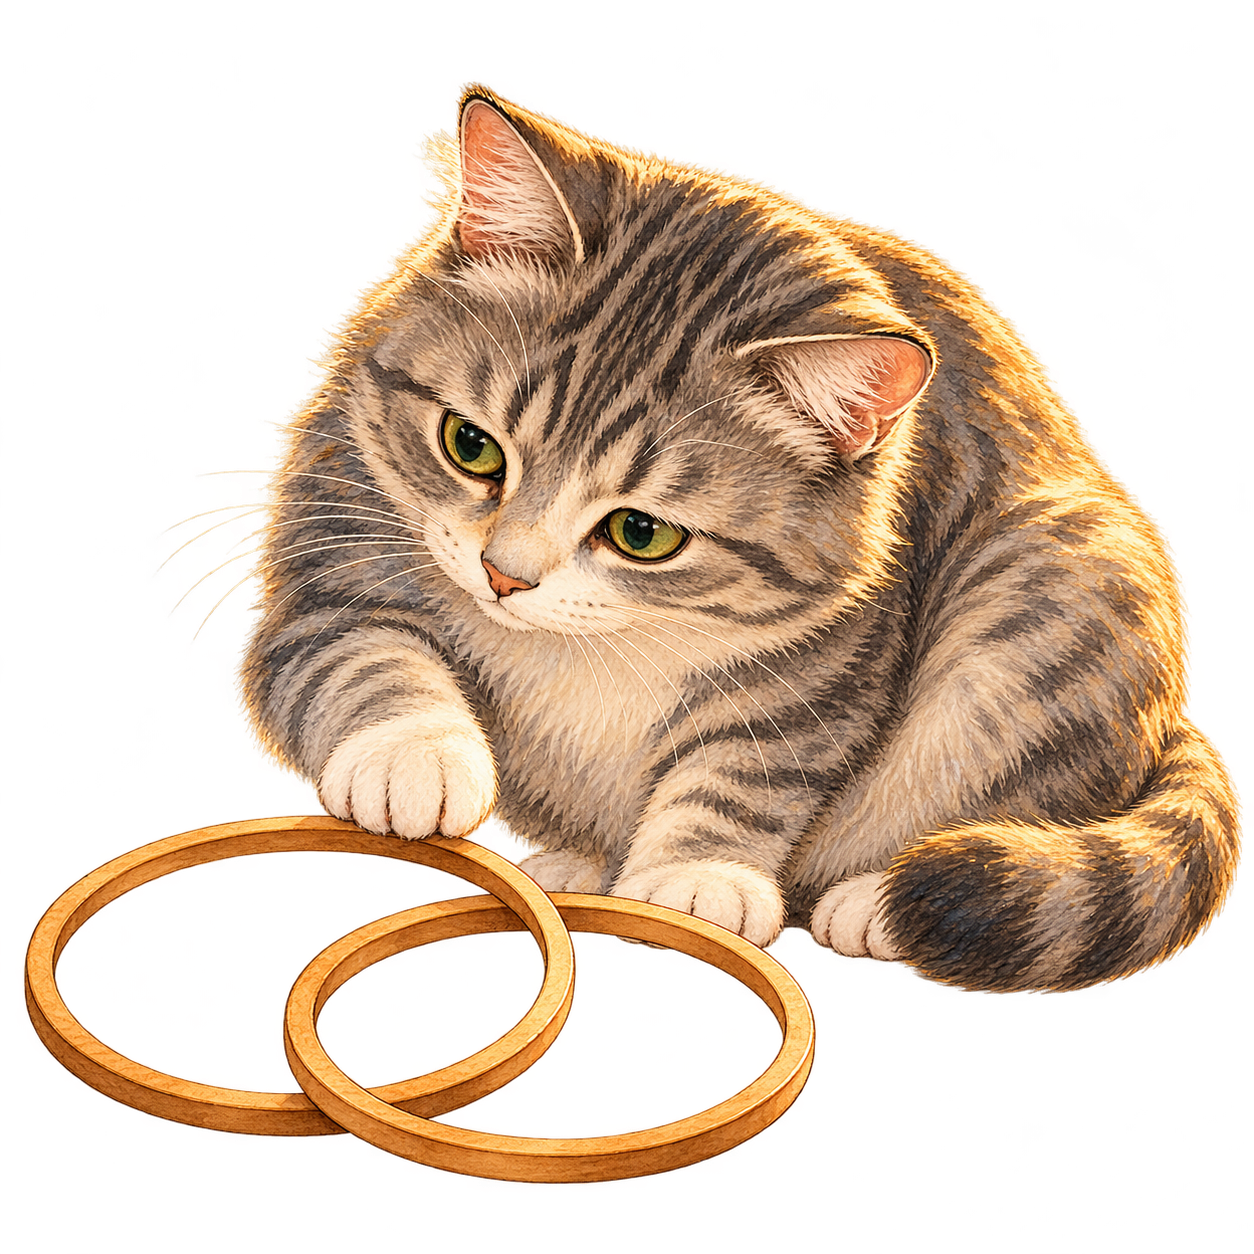
\includegraphics[width=54mm,height=58mm,keepaspectratio]{images/unique/art-32.png}
\label{catflow:32}
\end{wrapfigure}
\textbf{9.6.} Верна ли импликация: если число делится на \(4\), то оно чётное? Верно ли обратное?\par

\textbf{9.7.} Для делимости на \(6\) чётность — необходимое или достаточное условие?\par

\textbf{9.8.} Докажи, что сумма двух чётных целых чисел чётна.\par

\textbf{9.9.} Докажи, что квадрат нечётного целого числа нечётный.\par

\textbf{9.10.} Опровергни: если \(a^{2} = b^{2}\), то \(a = b\) для любых действительных \(a,\allowbreak b\).\par

\textbf{9.11.} Докажи по индукции: \(1 + 2 + \ldots  + n = \dfrac{n (n + 1)}{2}\) для натуральных \(n \ge  1\).\par

\textbf{9.12.} Докажи: если целое \(n\) нечётно, то \(n^{2}\) нечётно. Сформулируй равносильное утверждение через противоположное условие.\par
\par\WFclear\end{minipage}\end{lrbox}%
\ifdim\dimexpr\ht\CatFlowBox+\dp\CatFlowBox\relax<64mm\dp\CatFlowBox=\dimexpr64mm-\ht\CatFlowBox\relax\fi%
\noindent\usebox{\CatFlowBox}\par\addvspace{5pt}

\noindent\begin{minipage}[t]{\linewidth}\textbf{9.13.} В кафе все комплексные обеды включают напиток. Покупатель получил напиток. Обязательно ли он заказал комплексный обед?\par\end{minipage}\par
\noindent\begin{minipage}[t]{\linewidth}\textbf{9.14.} В группе \(20\) человек. Чай любят \(12\), кофе любят \(9\), оба напитка любят \(5\). Сколько любят хотя бы один из напитков и сколько не любят ни один?\par\end{minipage}\par
\noindent\begin{minipage}[t]{\linewidth}\textbf{9.15.} Объявление гласит: «Все автобусы на этом маршруте низкопольные». Какое наблюдение опровергнет утверждение? Сформулируй его отрицание.\par\end{minipage}\par
\noindent\begin{minipage}[t]{\linewidth}\textbf{9.16.}\starmark{} Из \(30\) учеников \(18\) изучают английский, \(16\) немецкий, каждый изучает хотя бы один из этих языков. Сколько изучают оба и сколько только английский?\begin{center}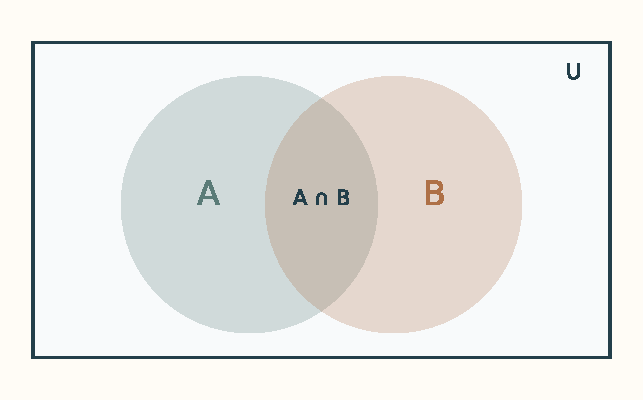
\includegraphics[width=.7\linewidth,height=45mm,keepaspectratio]{images/diagram-venn.pdf}\end{center}\par\end{minipage}\par
\noindent\begin{minipage}[t]{\linewidth}\textbf{9.17.}\starmark{} Докажи: если квадрат целого числа делится на \(3\), то само число делится на \(3\).\par\end{minipage}\par
\noindent\begin{minipage}[t]{\linewidth}\textbf{9.18.}\starmark{} Докажи по индукции: \(1 + 3 + 5 + \ldots  + (2 n - 1) = n^{2}\) для \(n \ge  1\).\par\end{minipage}\par
\noindent\begin{minipage}[t]{\linewidth}\textbf{9.19.}\starmark{} Для \(A,B\subseteq U\) докажи равенство \(A\setminus B=A\cap(U\setminus B)\) через принадлежность произвольного элемента.\par\end{minipage}\par
\noindent\begin{minipage}[t]{\linewidth}\textbf{9.20.}\starmark{} Докажи распределительный закон \(A\cap(B\cup C)=(A\cap B)\cup(A\cap C)\) через принадлежность элемента. Объясни, что нужно закрасить на диаграмме Венна для каждой стороны.\par\end{minipage}\par
\noindent\begin{minipage}[t]{\linewidth}\textbf{9.21.} Пусть \(A=\{1,2\}\), \(B=\{1,2,3\}\), \(C=\{2,4\}\). Определи истинность записей \(A\subseteq B\), \(A\subset B\), \(C\subseteq B\), \(\varnothing\subseteq A\).\par\end{minipage}\par
\noindent\begin{minipage}[t]{\linewidth}\textbf{9.22.} Выпиши все элементы \(\mathcal P(\{a,b\})\), где \(a\ne b\). Сколько подмножеств имеет множество из четырёх элементов?\par\end{minipage}\par
\noindent\begin{minipage}[t]{\linewidth}\textbf{9.23.} Даны \(U=\{1,2,3,4,5,6,7,8\}\), \(A=\{2,4,6,8\}\), \(B=\{1,2,3,4\}\). Найди \(A\setminus B\), \(B\setminus A\), \(A\triangle B\), \(U\setminus A\), \(U\setminus B\).\par\end{minipage}\par
\noindent\begin{minipage}[t]{\linewidth}\textbf{9.24.} При \(A=\{1,2\}\), \(B=\{3\}\) выпиши \(A\times B\) и \(B\times A\). Равны ли эти множества? Сколько элементов в каждом?\par\end{minipage}\par
\noindent\begin{minipage}[t]{\linewidth}\textbf{9.25.} В группе пять человек: Аня, Боря, Вера, Глеб и Даша. Английским занимаются Аня, Вера и Даша, музыкой — Боря и Вера. Кто посещает ровно одно из двух занятий? Кто не посещает ни одно? Запиши ответы как симметрическую разность и дополнение объединения.\par\end{minipage}\par
\noindent\begin{minipage}[t]{\linewidth}\textbf{9.26.}\starmark{} Команду выбирают из шести человек: Ани, Бори, Веры, Глеба, Даши и Егора. Аня и Боря обязательно входят в команду, Вера не входит, а остальных можно включать или не включать. Сколько разных команд возможно? Объясни связь с множеством всех подмножеств.\par\end{minipage}\par
\par\addvspace{5pt}\begin{lrbox}{\CatFlowBox}\begin{minipage}[t]{\linewidth}
\setlength{\parskip}{5pt}\setlength{\columnsep}{4.5mm}\setlength{\intextsep}{0pt}
\begin{wrapfigure}[13]{l}{54mm}

\includegraphics[width=54mm,height=58mm,keepaspectratio]{images/unique/art-83.png}
\label{catflow:83}
\end{wrapfigure}
\textbf{9.27.} При \(v(p)=1,v(q)=0,v(r)=1\) вычисли значения \((p\lor q)\land\neg r\), \((p\uparrow q)\to r\) и \((p\oplus r)\downarrow q\).\par

\textbf{9.28.} Построй таблицу истинности формулы \((p\to q)\leftrightarrow(\neg q\to\neg p)\). Является ли она тавтологией?\par

\textbf{9.29.} Для каждой формулы \(p\lor\neg p\), \(p\land\neg p\), \(p\oplus q\) определи: тавтология, противоречие или ни то ни другое. Для последнего случая предъяви оценки с разными результатами.\par

\textbf{9.30.} Запиши формулу \((p\to q)\land(q\to p)\), используя только \(\neg,\land,\lor\). Объясни её связь с \(p\leftrightarrow q\).\par

\textbf{9.31.} Проверь два семантических следования: \(\{p\lor q\}\models p\) и \(\{p\land q\}\models p\lor r\). Неверное опровергни контроценкой, верное обоснуй для произвольной оценки с истинной посылкой.\par

\textbf{9.32.} Преобразуй отрицание \(\neg((p\lor q)\land r)\) в равносильную формулу, где отрицания стоят только перед переменными. Обоснуй каждое применение закона де Моргана.\par
\par\WFclear\end{minipage}\end{lrbox}%
\ifdim\dimexpr\ht\CatFlowBox+\dp\CatFlowBox\relax<64mm\dp\CatFlowBox=\dimexpr64mm-\ht\CatFlowBox\relax\fi%
\noindent\usebox{\CatFlowBox}\par\addvspace{5pt}

\noindent\begin{minipage}[t]{\linewidth}\textbf{9.33.} В упрощённой модели дверь открыта тогда и только тогда, когда действителен пропуск \(p\), введён верный PIN-код \(q\) и не включена аварийная блокировка \(r\). Обозначь открытое состояние через \(o\), запиши правило формулой и найди \(o\) при тройках \((p,q,r)=(1,1,0),(1,0,0),(1,1,1)\). Доказывает ли закрытая дверь, что блокировка включена?\par\end{minipage}\par
\noindent\begin{minipage}[t]{\linewidth}\textbf{9.34.} Лампа горит ровно тогда, когда два переключателя находятся в разных положениях. Их положения обозначены \(p,q\), состояние лампы — \(l\). Запиши правило. Докажи по двум возможным случаям, что изменение положения ровно одного переключателя всегда меняет состояние лампы.\par\end{minipage}\par
\noindent\begin{minipage}[t]{\linewidth}\textbf{9.35.} Построй формальный вывод \(\Gamma\vdash q\land r\), где \(\Gamma=\{p\land q,p\to r\}\). Укажи правило каждого шага.\par\end{minipage}\par
\noindent\begin{minipage}[t]{\linewidth}\textbf{9.36.} Докажи формально \(\vdash p\to(q\to p)\). Объясни, какие предположения снимаются и почему предположение \(q\) можно снять, даже если оно не понадобилось.\par\end{minipage}\par
\noindent\begin{minipage}[t]{\linewidth}\textbf{9.37.} При \(\Gamma=\{p\to q,q\to r\}\) выведи \(\Gamma\vdash p\to r\). Временно добавь \(p\) и укажи оба применения modus ponens.\par\end{minipage}\par
\noindent\begin{minipage}[t]{\linewidth}\textbf{9.38.}\starmark{} При \(\Gamma=\{p\lor q,p\to r,q\to r\}\) построй вывод \(\Gamma\vdash r\) разбором случаев. Почему нельзя просто выбрать одну часть дизъюнкции?\par\end{minipage}\par
\noindent\begin{minipage}[t]{\linewidth}\textbf{9.39.}\starmark{} Построй формальный вывод \(\vdash(p\land(q\lor r))\to((p\land q)\lor(p\land r))\). Используй устранение конъюнкции, разбор случаев и снятие временных предположений.\par\end{minipage}\par
\noindent\begin{minipage}[t]{\linewidth}\textbf{9.40.} Ученик предлагает вывод: «Даны \(p\to q\) и \(q\); значит, по modus ponens получаем \(p\)». Найди ошибку и с помощью контроценки и теоремы о сохранении истины докажи, что \(\{p\to q,q\}\vdash p\) вообще не имеет вывода по выбранным правилам.\par\end{minipage}\par
\noindent\begin{minipage}[t]{\linewidth}\textbf{9.41.}\starmark{} Используя только связку NAND, построй формулы, равносильные \(\neg p\), \(p\land q\) и \(p\lor q\). Для каждой формулы объясни равносильность через определение \(\uparrow\).\par\end{minipage}\par
\noindent\begin{minipage}[t]{\linewidth}\textbf{9.42.}\starmark{} Построй формулу для \(p\oplus q\), используя только NOR. Можно ввести промежуточные формулы. Проверь результат таблицей с четырьмя входными наборами.\par\end{minipage}\par
\endgroup
